\PassOptionsToPackage{unicode=true}{hyperref} % options for packages loaded elsewhere
\PassOptionsToPackage{hyphens}{url}
%
\documentclass[ignorenonframetext,]{beamer}
\usepackage{pgfpages}
\setbeamertemplate{caption}[numbered]
\setbeamertemplate{caption label separator}{: }
\setbeamercolor{caption name}{fg=normal text.fg}
\beamertemplatenavigationsymbolsempty
% Prevent slide breaks in the middle of a paragraph:
\widowpenalties 1 10000
\raggedbottom
\setbeamertemplate{part page}{
\centering
\begin{beamercolorbox}[sep=16pt,center]{part title}
  \usebeamerfont{part title}\insertpart\par
\end{beamercolorbox}
}
\setbeamertemplate{section page}{
\centering
\begin{beamercolorbox}[sep=12pt,center]{part title}
  \usebeamerfont{section title}\insertsection\par
\end{beamercolorbox}
}
\setbeamertemplate{subsection page}{
\centering
\begin{beamercolorbox}[sep=8pt,center]{part title}
  \usebeamerfont{subsection title}\insertsubsection\par
\end{beamercolorbox}
}
\AtBeginPart{
  \frame{\partpage}
}
\AtBeginSection{
  \ifbibliography
  \else
    \frame{\sectionpage}
  \fi
}
\AtBeginSubsection{
  \frame{\subsectionpage}
}
\usepackage{lmodern}
\usepackage{amssymb,amsmath}
\usepackage{ifxetex,ifluatex}
\usepackage{fixltx2e} % provides \textsubscript
\ifnum 0\ifxetex 1\fi\ifluatex 1\fi=0 % if pdftex
  \usepackage[T1]{fontenc}
  \usepackage[utf8]{inputenc}
  \usepackage{textcomp} % provides euro and other symbols
\else % if luatex or xelatex
  \usepackage{unicode-math}
  \defaultfontfeatures{Ligatures=TeX,Scale=MatchLowercase}
\fi
\usetheme[]{Frankfurt}
% use upquote if available, for straight quotes in verbatim environments
\IfFileExists{upquote.sty}{\usepackage{upquote}}{}
% use microtype if available
\IfFileExists{microtype.sty}{%
\usepackage[]{microtype}
\UseMicrotypeSet[protrusion]{basicmath} % disable protrusion for tt fonts
}{}
\IfFileExists{parskip.sty}{%
\usepackage{parskip}
}{% else
\setlength{\parindent}{0pt}
\setlength{\parskip}{6pt plus 2pt minus 1pt}
}
\usepackage{hyperref}
\hypersetup{
            pdftitle={Clojure programming language \& it's ecosystem},
            pdfauthor={Marius Rabenarivo},
            pdfborder={0 0 0},
            breaklinks=true}
\urlstyle{same}  % don't use monospace font for urls
\newif\ifbibliography
\usepackage{graphicx,grffile}
\makeatletter
\def\maxwidth{\ifdim\Gin@nat@width>\linewidth\linewidth\else\Gin@nat@width\fi}
\def\maxheight{\ifdim\Gin@nat@height>\textheight\textheight\else\Gin@nat@height\fi}
\makeatother
% Scale images if necessary, so that they will not overflow the page
% margins by default, and it is still possible to overwrite the defaults
% using explicit options in \includegraphics[width, height, ...]{}
\setkeys{Gin}{width=\maxwidth,height=\maxheight,keepaspectratio}
\setlength{\emergencystretch}{3em}  % prevent overfull lines
\providecommand{\tightlist}{%
  \setlength{\itemsep}{0pt}\setlength{\parskip}{0pt}}
\setcounter{secnumdepth}{0}

% set default figure placement to htbp
\makeatletter
\def\fps@figure{htbp}
\makeatother


\title{Clojure programming language \& it's ecosystem}
\author{Marius Rabenarivo}
\date{}
\titlegraphic{
\includegraphics{MSCC-DevCon2024-logo.png}}

\begin{document}
\frame{\titlepage}

\begin{frame}{What is Clojure?}
\protect\hypertarget{what-is-clojure}{}

\begin{itemize}
\tightlist
\item
  LISP
\end{itemize}

\begin{figure}
\centering
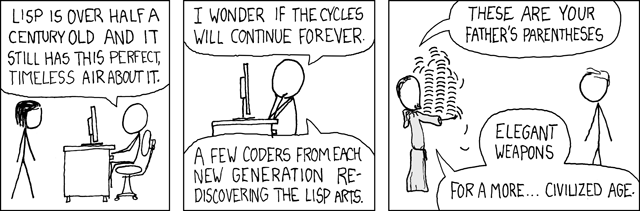
\includegraphics[width=1.5625in,height=\textheight]{lisp_cycles.png}
\caption{Lisp Cycles, https://xkcd.com/297/}
\end{figure}

\begin{itemize}
\tightlist
\item
  Rich Hickey
\end{itemize}

\begin{figure}
\centering
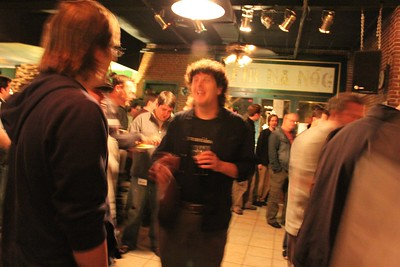
\includegraphics[width=1.5625in,height=\textheight]{rich-hickey-clojure-conj-2010.jpg}
\caption{Rich Hickey at the first Clojure Conj in 2010,
https://creativecommons.org/licenses/by-sa/2.0/}
\end{figure}

\begin{itemize}
\tightlist
\item
  General Purpose
\end{itemize}

\end{frame}

\begin{frame}{What is LISP?}
\protect\hypertarget{what-is-lisp}{}

\begin{figure}
\centering
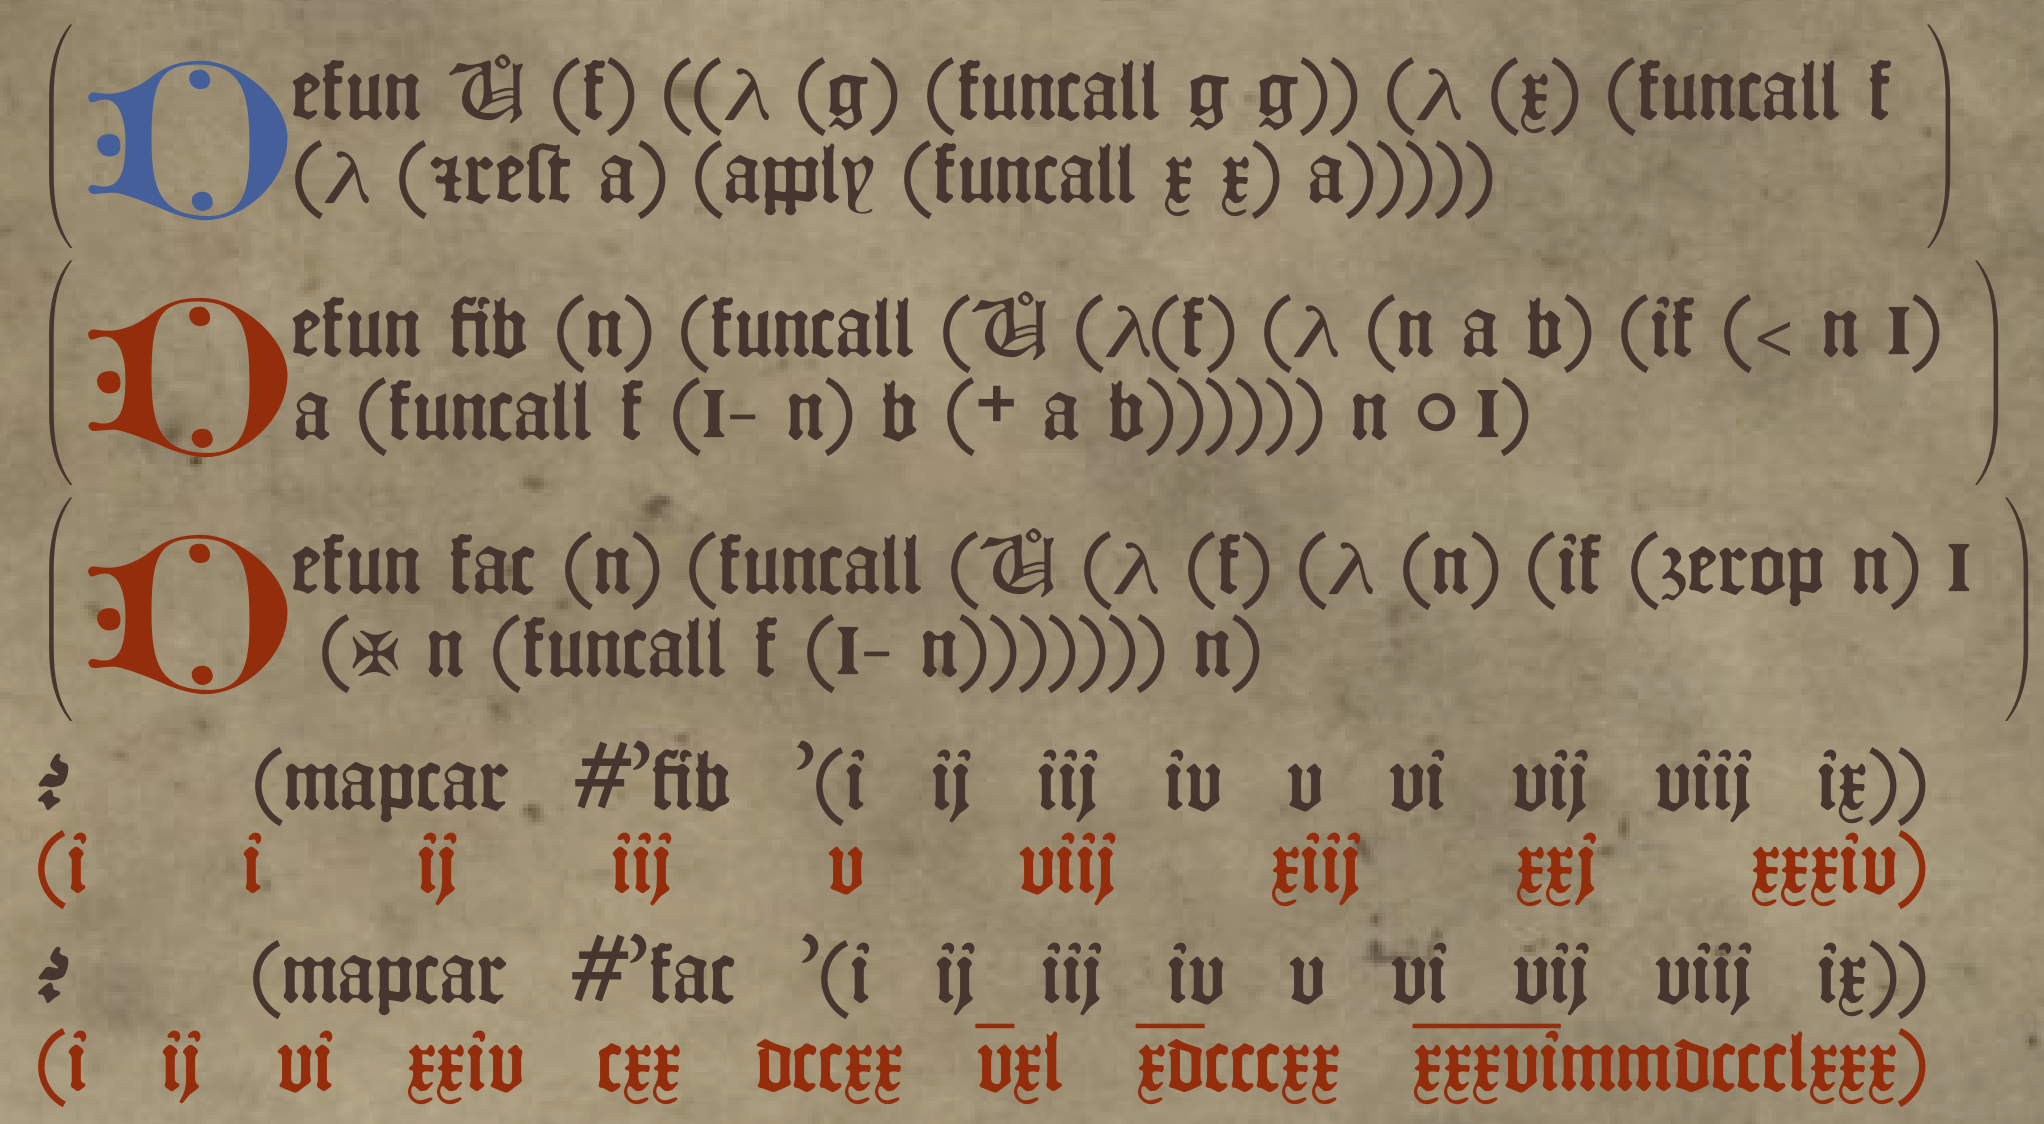
\includegraphics{ycombinator-codex_banner.png}
\caption{Y Combinator Codex by emacsomancer.}
\end{figure}

\end{frame}

\begin{frame}{What is LISP?}
\protect\hypertarget{what-is-lisp-1}{}

\begin{itemize}
\tightlist
\item
  LISt Processing language
\item
  2nd oldest High-Level Language after FORTRAN
\item
  1958 - John McCarthy
\end{itemize}

\begin{figure}
\centering
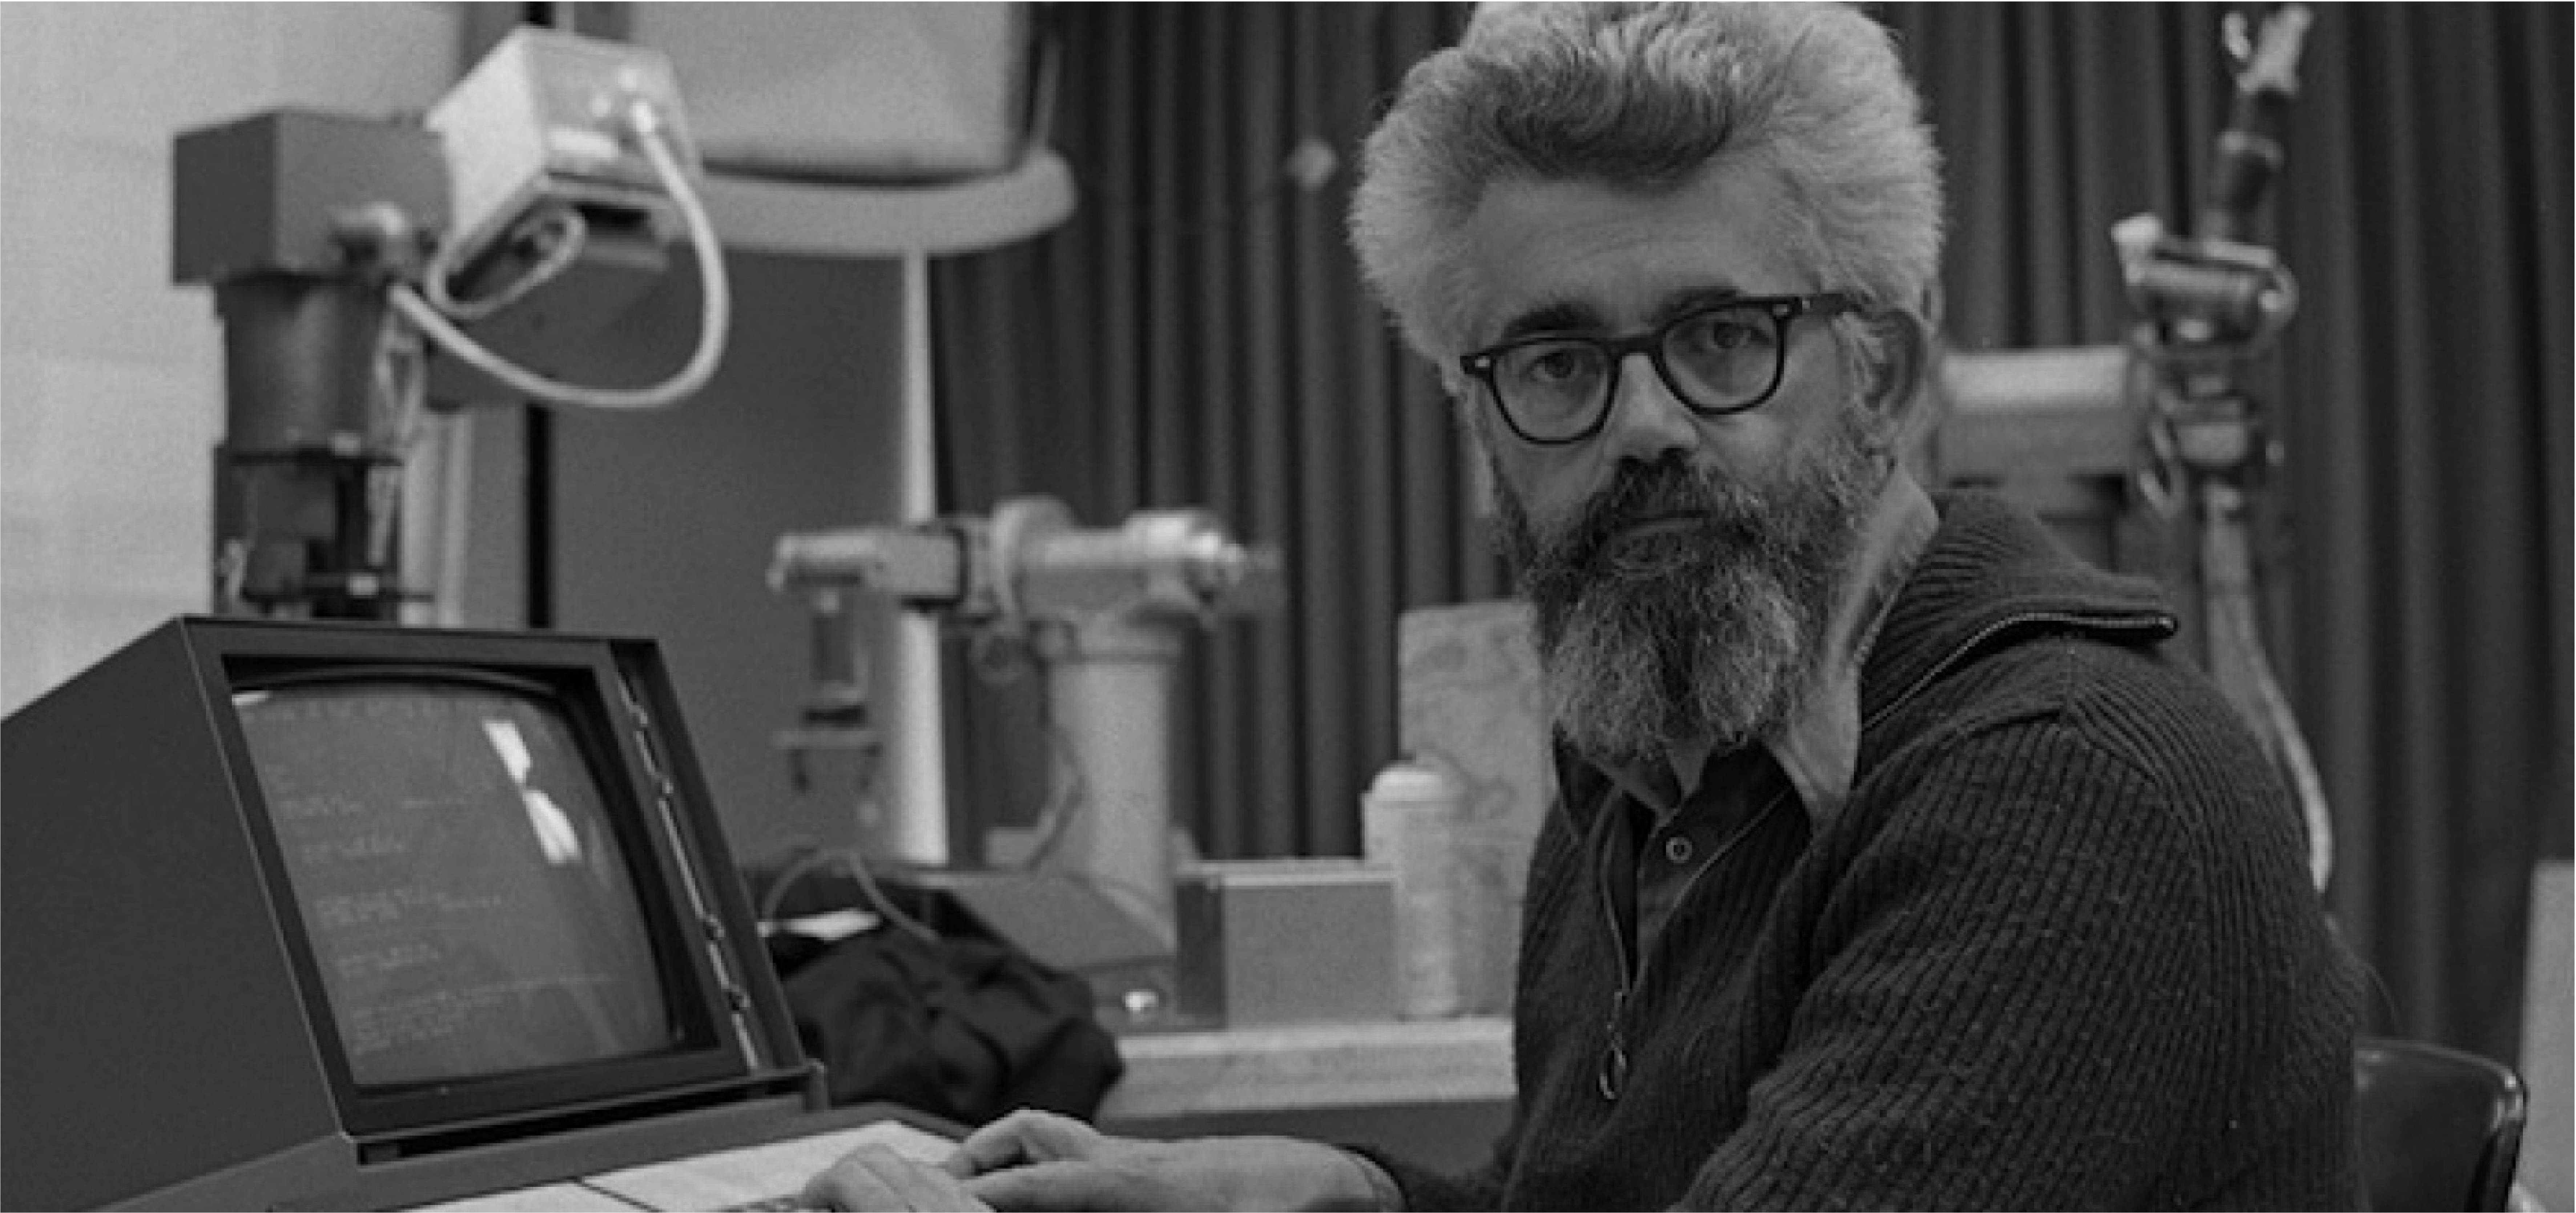
\includegraphics{john_mccarthy.jpg}
\caption{John McCarthy at work in his artificial intelligence laboratory
at Stanford}
\end{figure}

\end{frame}

\begin{frame}{Why Clojure?}
\protect\hypertarget{why-clojure}{}

\begin{itemize}
\tightlist
\item
  Designed with simplicity
\item
  Functional Programming
\item
  Data Oriented
\end{itemize}

\begin{figure}
\centering

\includegraphics[width=3.75in,height=\textheight]{spiderman-pointing-meme.jpg}
\caption{Code? Data? Code? Data?}
\end{figure}

\end{frame}

\begin{frame}{Why Clojure?}
\protect\hypertarget{why-clojure-1}{}

\begin{figure}
\centering
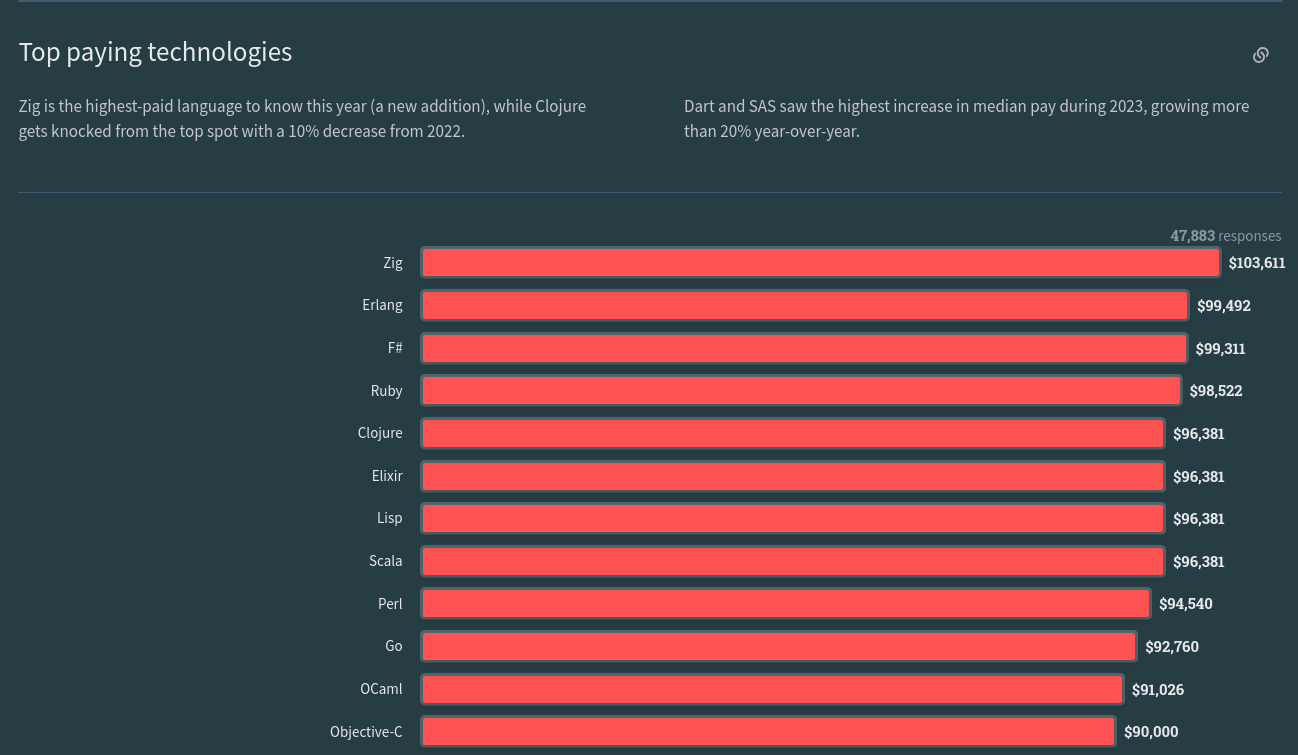
\includegraphics[width=\textwidth,height=2.5in]{Stack-Overflow-Developer-Survey-2023-top-paying-technologies.png}
\caption{2023 Developer Survey, Top paying technologies}
\end{figure}

\textbf{Source:}
\url{https://survey.stackoverflow.co/2023/\#section-top-paying-technologies-top-paying-technologies}

\end{frame}

\begin{frame}{Why Clojure?}
\protect\hypertarget{why-clojure-2}{}

\begin{figure}
\centering
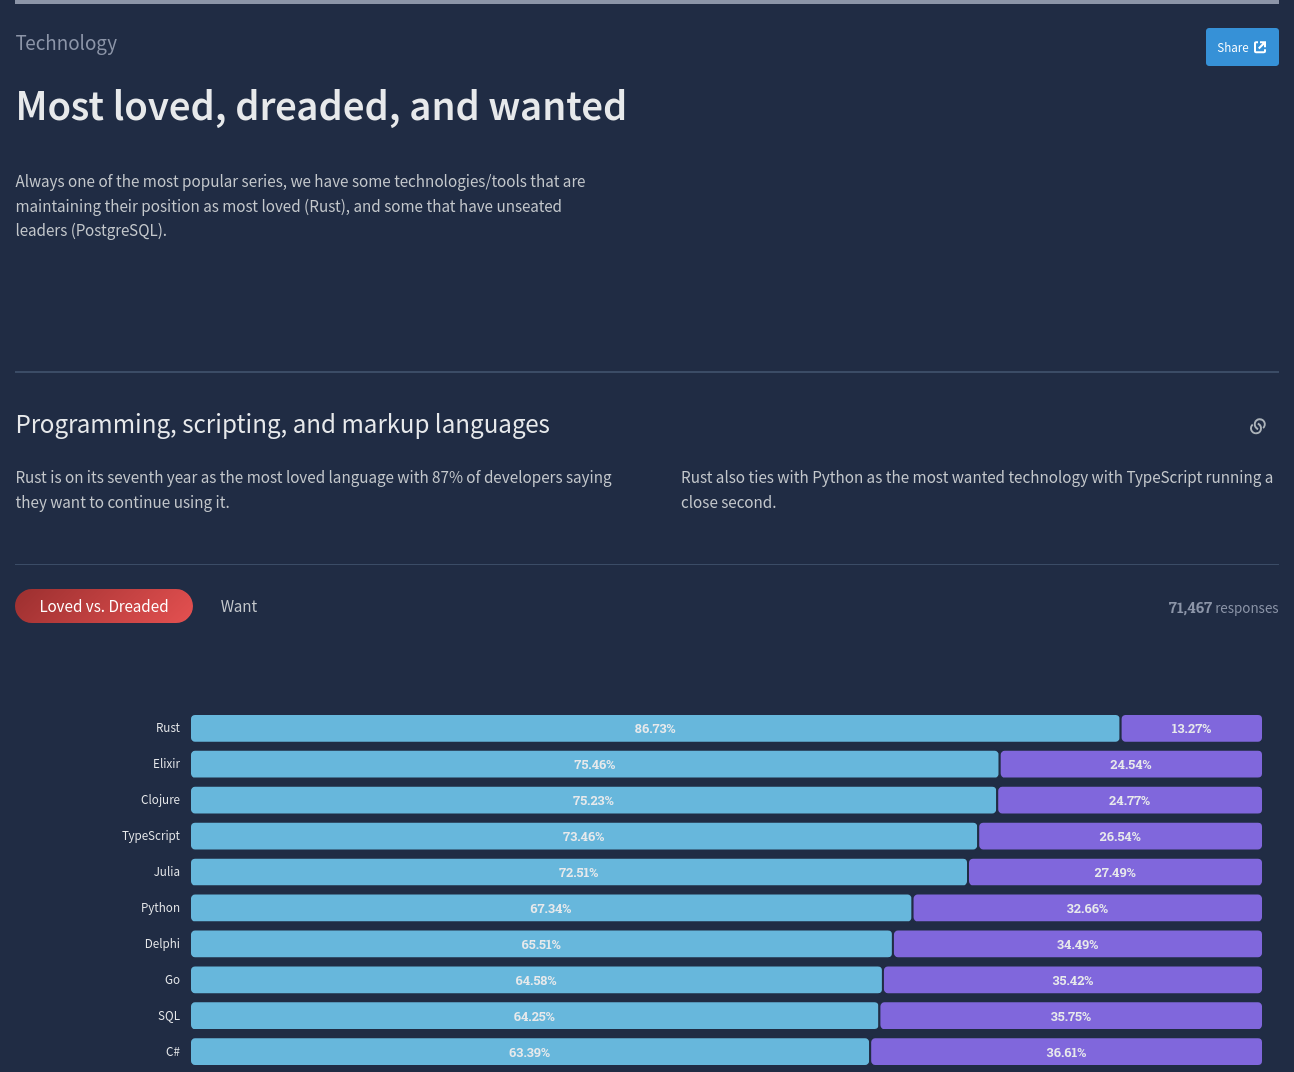
\includegraphics[width=\textwidth,height=2.5in]{Stack-Overflow-Developer-Survey-2022-most-loved-dreaded-and-wanted-language-love-dread.png}
\caption{Stack Overflow Developer Survey 2022, Most loved, dreaded, and
wanted}
\end{figure}

\textbf{Source:}
\url{https://survey.stackoverflow.co/2022/\#technology-most-loved-dreaded-and-wanted}

\end{frame}

\begin{frame}{Functional Programming}
\protect\hypertarget{functional-programming}{}

\begin{itemize}
\tightlist
\item
  Immutability
\item
  Referential transparency
\item
  Easy to think about systems
\item
  Parallel and concurrent programming
\end{itemize}

\end{frame}

\end{document}
